% Context evolution section (Sun). Drop-in for the team NeurIPS template; figures in figures/.
% Numbers: Situation Puzzles, 100 official test puzzles, paired by puzzle, seeds averaged within puzzle,
% 95% bootstrap confidence intervals over puzzles. Source tables: experiments/13_sp_context_evolution/RESULTS.md.

\section{Context Evolution}
\label{sec:context}

Harness search changes the code around a frozen model. Context evolution changes only the text the model reads:
a playbook of rules, or a memory of past episodes. We ask the same question as in the rest of the paper, now in this
medium. Can a frozen Qwen2.5-7B-Instruct improve at Situation Puzzles (SP) from its own experience, if all it can change
is its context?

\subsection{Setup}

\paragraph{Task and models.} The agent asks up to 25 questions about a puzzle and then writes the hidden story. A
referee (Qwen3-235B-A22B) answers each question with Yes, No or Unknown from the hidden story. We split the official
SP training file into 300 TRAIN and 100 VAL puzzles and report on the 100 official test puzzles, with 3 to 5 seeds per
method. One episode costs 51 calls (25 questions, 25 referee answers, 1 final answer).

\paragraph{Two scores.} \emph{Question recall} is the share of the hidden story's key points that the questions
uncover; it measures information acquisition. \emph{Story score} is the number of key points (0 to 6) that the final
story matches, using the AR-Bench grading prompt; it is the task score.

\paragraph{Two judges.} Both scores need an LLM judge. Our first judge (Claude Haiku 5.5) turned out to be lenient:
on 100 items it agreed with a stronger reference grader (Claude Opus 5.5) 80 times, against 91 of 98 for Gemini 3.7
Flash. When the two judges disagreed, the reference grader sided with Haiku in 33 to 50\% of the cases that only Haiku
credited, and with Gemini in 77 to 84\% of the cases that only Gemini credited. We therefore report both judges and
treat a result as real only if it holds under the stricter one.

\subsection{Evolving the questioning playbook does not transfer to test}

We evolved a playbook of questioning rules for 4 rounds (answer, then evolve, then answer again) with several kinds
of experience: contrasting successful and failed episodes, step-level credit from asking alternative questions at
the same state (and the same credit randomly shuffled, as a control), and a prior over common hidden stories. A
candidate playbook is kept only if it raises VAL recall. We also ran two open-source methods, ACE and Dynamic
Cheatsheet, and the Bayesian question-selection method BALAR.

Validation recall rises in every run (Figure~\ref{fig:rounds}, left). On test, no evolved playbook beats the empty one
under the strict judge (Figure~\ref{fig:judgegap}). The lenient judge shows small gains (+0.029 for the
success/failure contrast), which disappear under the strict judge ($-0.007$, CI $[-0.041, +0.027]$). Selecting
playbooks with the strict judge, or with both judges at once, removes the lenient-judge gain but does not produce a
test gain either (Figure~\ref{fig:rounds}, right). ACE, which learns from judge feedback, is worse than the empty
playbook under the strict judge ($-0.050$, $[-0.083, -0.017]$); Dynamic Cheatsheet is flat ($-0.014$). Writing the
choices of best-of-8 sampling into rules hurts ($-0.071$). The real and the shuffled step-level credit give the same
playbook quality, so the counterfactual signal itself adds nothing here. BALAR (1 seed) reaches a recall of 0.355
against 0.386 for the empty playbook, at about 297 calls per episode.

Our reading is that the evolution loop is doing what it is asked to do: it raises the score used for selection. With a
lenient judge, part of that score is the judge's leniency, and with 60 VAL puzzles, part of it is noise. This matches
the overfitting to the validation set that we see for harness search.

\begin{figure}[t]
  \centering
  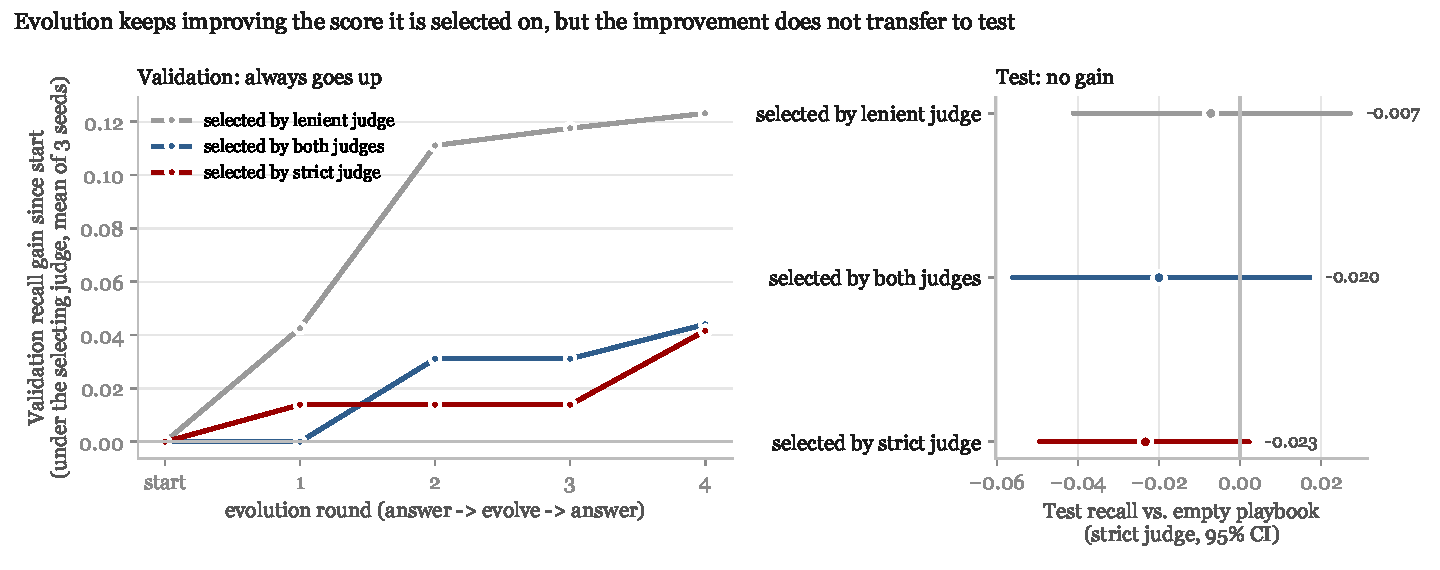
\includegraphics[width=\linewidth]{figures/figD_rounds_vs_test.pdf}
  \caption{Left: VAL recall gain over the starting playbook in each evolution round, under the judge used to select
  playbooks (mean of 3 seeds). Right: test recall against the empty playbook under the strict judge.}
  \label{fig:rounds}
\end{figure}

\begin{figure}[t]
  \centering
  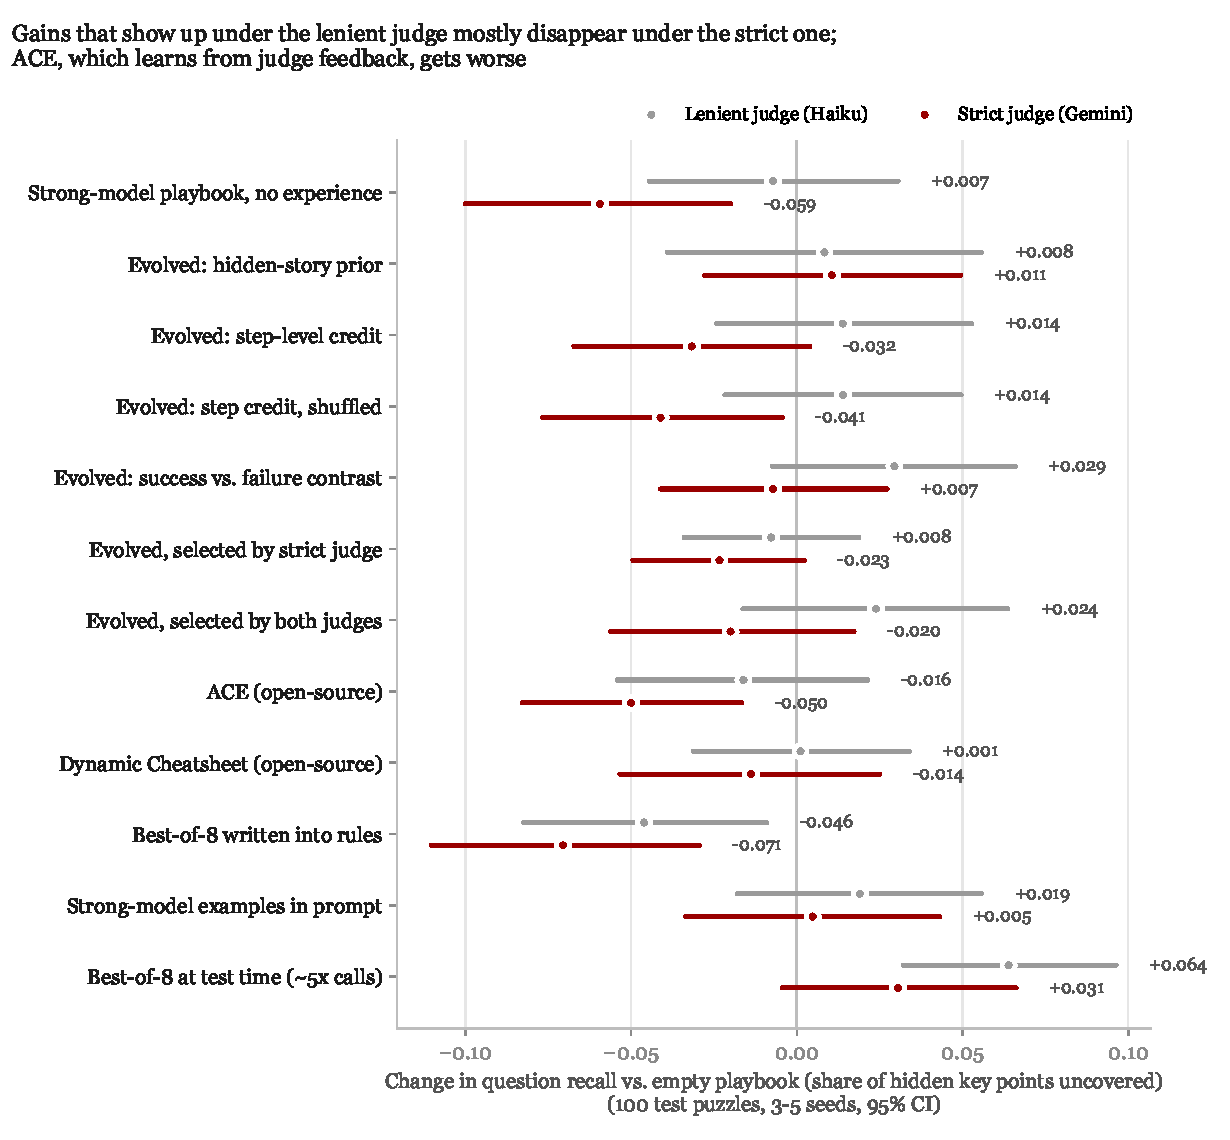
\includegraphics[width=0.92\linewidth]{figures/figC_judge_gap.pdf}
  \caption{Change in test question recall against the empty playbook, under each judge (100 puzzles, 3 to 5 seeds,
  95\% CI). Test-time best-of-8 is shown for reference; it costs about five times as many calls.}
  \label{fig:judgegap}
\end{figure}

\subsection{Both asking and using are bottlenecks}

To see where the 7B loses points, we swapped one side of the episode at a time (test, seed 0). Keeping the 7B's own
questions and letting a stronger model (Claude Opus 5.5) write the final story raises the story score from 0.50 to
1.56 under the strict judge (0.77 to 2.06 under the lenient one). Letting Qwen3-235B ask the questions and the 7B write
the story raises it to 1.33 (strict; 1.82 lenient) (Figure~\ref{fig:askuse}). Both sides matter, and the use side is large: the 7B's questions already uncover about 2.3
to 2.7 of the 6 key points, but its story matches fewer than one.

\begin{figure}[t]
  \centering
  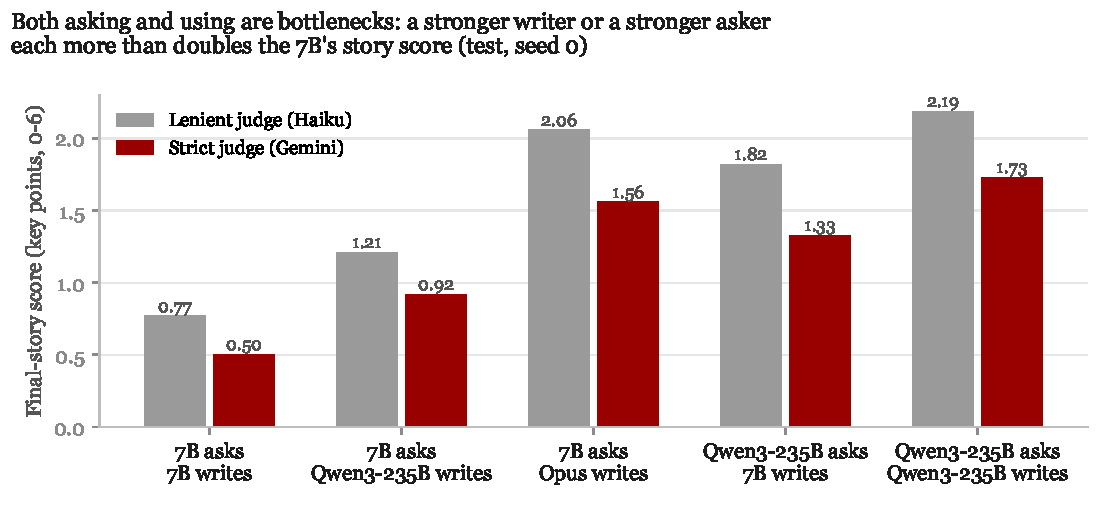
\includegraphics[width=0.8\linewidth]{figures/figE_ask_vs_use.pdf}
  \caption{Story score when a stronger model asks the questions or writes the final story (test, seed 0).}
  \label{fig:askuse}
\end{figure}

\subsection{A memory of past puzzles, used at the answer step, helps under both judges}

Since the questioning playbook did not transfer, we moved the context to the step where the information is used.
Before the 7B writes its final story, we show it two TRAIN puzzles from its own past episodes: the puzzle, the
questions and answers from that episode, and the true hidden story. The 7B, the transcript and the final prompt are
unchanged. Examples are retrieved by the similarity of the puzzle text only, so no test answer is used. As a control
we resample the final answer from the same transcript without examples.

The memory raises the story score by 0.25 (lenient, $[+0.16, +0.35]$) and 0.17 (strict, $[+0.08, +0.26]$), from
0.49 to 0.67 under the strict judge (Figure~\ref{fig:answerstep}). Three ablations explain where this comes from.
\begin{itemize}
  \item \textbf{The true story is necessary.} The same two examples without their stories give no gain ($-0.03$
  strict).
  \item \textbf{Similarity helps, but is not required.} Two random past puzzles still help ($+0.10$ strict,
  $[+0.03, +0.17]$), and so do examples with all near-variant puzzles removed ($+0.13$ lenient, $+0.08$ strict,
  $[-0.01, +0.16]$).
  \item \textbf{Part of the gain comes from puzzle families.} SP contains near variants of the same puzzle across
  train and test (for example, several puzzles about a letter that arrives after the writer's funeral). The extra
  gain of similar over random examples comes from the third of test puzzles whose nearest TRAIN story is closest
  (Figure~\ref{fig:where}).
\end{itemize}
Examples whose questions were asked by a stronger model (Qwen3-235B) give the same gain as the 7B's own (+0.20 strict). Asking the 7B to
list the confirmed facts before writing helps less (+0.09 strict). Putting the same kind of examples in the system
prompt during questioning does not raise question recall under the strict judge (+0.005); the story score rises
(+0.17 strict) but its interval includes zero. We read this as the 7B learning from the examples how to combine confirmed facts into one
story, which is the use-side gap found above.

\begin{figure}[t]
  \centering
  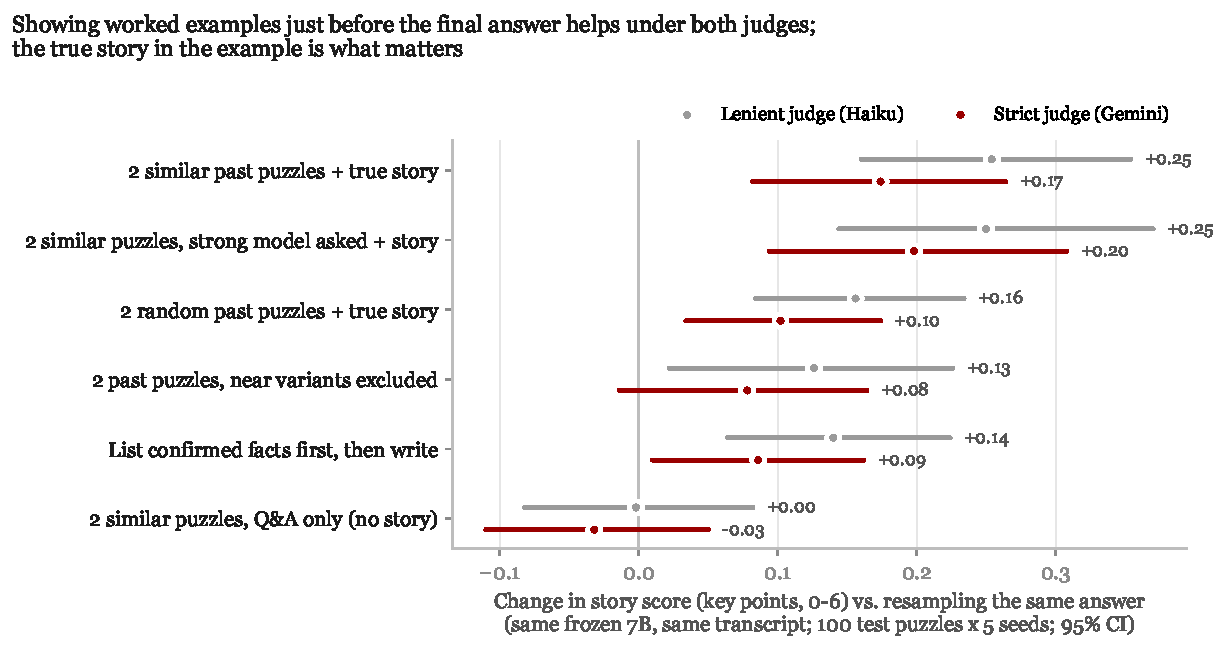
\includegraphics[width=0.92\linewidth]{figures/figA_answer_step.pdf}
  \caption{Change in story score against resampling the same final answer (same 7B and transcript, 100 test puzzles
  $\times$ 5 seeds, 95\% CI).}
  \label{fig:answerstep}
\end{figure}

\begin{figure}[t]
  \centering
  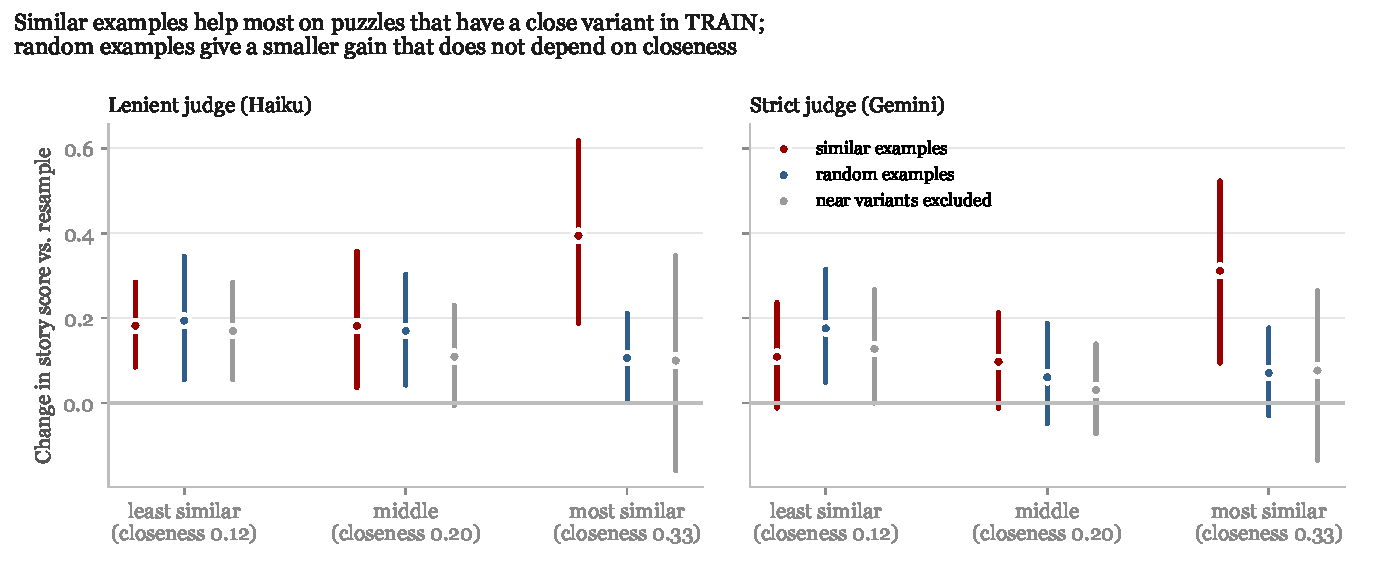
\includegraphics[width=\linewidth]{figures/figB_where_gain_comes_from.pdf}
  \caption{Answer-step gain by thirds of test puzzles, sorted by how close the nearest TRAIN puzzle's story is to the
  test story (used for this analysis only).}
  \label{fig:where}
\end{figure}

\subsection{Limitations}

All grading is done by LLM judges; we have no human labels. The absolute gain is small (under 0.3 of 6 key points). We
ran the answer-step memory on SP only. Part of the gain from similar examples comes from near-variant puzzles in the
benchmark, so we report the random-example result as the conservative estimate.
